\documentclass{beamer}
\usepackage[utf8]{inputenc}
\usepackage[T1]{fontenc}
\usepackage{amsmath}
\usepackage{graphicx}
\usepackage{lmodern}
\usepackage{listings}
\usepackage{xcolor}
\usepackage{hyperref}

\graphicspath{{img/}}
\setbeamertemplate{footline}[frame number]
\lstset{
    basicstyle=\ttfamily\footnotesize,
    keywordstyle=\color{blue},
    stringstyle=\color{red},
    showstringspaces=false
}
\hypersetup{
    colorlinks=true,
    linkcolor=blue,
    filecolor=magenta,
    urlcolor=cyan,
    pdftitle={Présentation — Méthode SIFT},
    pdfpagemode=FullScreen,
}

\title{Taitement d'image: SIFT}
\subtitle{Projet TIM}
\author{Louis LENOBLE, Raphael ROGER, Dylan SANSON, Jack SU}
\date{\today}

% Mini-sommaire automatique à chaque début de sous-section
\AtBeginSubsection[]{
  \begin{frame}{Sommaire}
    \tableofcontents[currentsection, currentsubsection]
  \end{frame}
}

\setcounter{tocdepth}{2}

\begin{document}

\begin{frame}
    \titlepage
\end{frame}

% Sommaire global
\begin{frame}{Sommaire}
    \tableofcontents
\end{frame}

\section{Qu'est ce que SIFT ?}
\subsection{Origines}
\begin{frame}{Origines}
    Le détecteur de coins de Harris-Stephens présente un défaut majeur : les coins qu'il localise sont invariant par rotation, mais pas par changement d'échelle.
    \begin{figure}
        \centering
        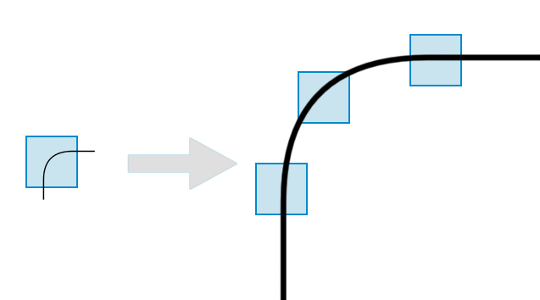
\includegraphics[width=0.58\textwidth]{img/harris_limites.png}
        \caption{Limites du détecteur de Harris-Stephens}
    \end{figure}
    Pour pouvoir repérer les coins à différentes échelles, on doit alors adapter la taille de la fenêtre utilisée par le détecteur de Harris-Stephens : c'est une tâche fastidieuse et difficile.
\end{frame}

\subsection{Signification}
\begin{frame}{Signification}
    SIFT signifie Scale-Invariant Feature Transform, c’est-à-dire une transformation de caractéristiques invariante à l’échelle.
\end{frame}

\subsection{Définition}
\begin{frame}{Définition}

    C'est une méthode développée en 1999. Elle permet d'extraire des features (ou points d'intérêt) de l'image et de \textbf{calculer leurs descripteurs}. 
    \\[1cm]
    Descripteur : Vecteur qui décrit le voisinage de la feature à laquelle il est associé. Il est utilisé dans le pattern matching pour repérer les paires de features qui se ressemblent le plus dans deux images.
\end{frame}

\section{Principe de SIFT}
\subsection{Les 4 étapes de SIFT}
\begin{frame}{Les 4 étapes principales de SIFT}
    L’algorithme SIFT implémenté dans le papier repose sur quatre étapes essentielles:
    \begin{itemize}
         \item Scale space extrema detection  
         \item Keypoint Localization
         \item Orientation Assignment
         \item Keypoint Descriptor
    \end{itemize}
\end{frame}

\subsection{Scale space extrema detection}
\subsubsection{Définition}
\begin{frame}{Scale space extrema detection}
    La première étape consiste à détecter les features/keypoints de l'image. Chaque feature est une zone circulaire intéressante, repérée par son centre et dont le rayon est proportionnel à son échelle caractéristique. La force du détecteur SIFT est sa capacité à trouver des features de différentes tailles.
    \\[1cm]
     \begin{itemize}
         \item Création d'une pyramide gaussienne  
         \item DoG de la pyramide gaussienne
         \item Recherche d'extremum locaux
     \end{itemize}
\end{frame}

\subsubsection{Pyamide Gaussienne et DoG}
\begin{frame}{Pyramide Gaussienne et DoG}
    \begin{figure}
        \centering
        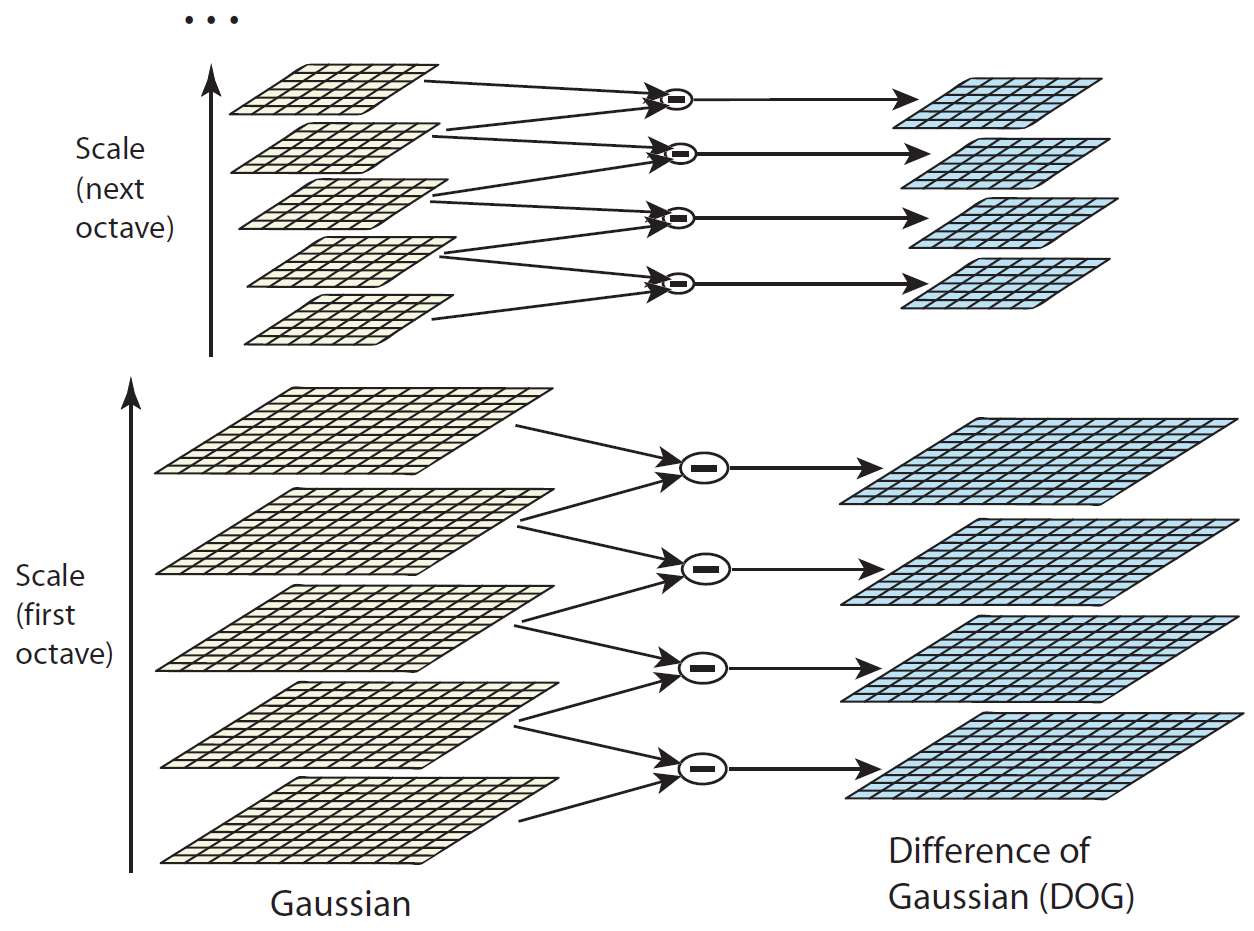
\includegraphics[width=0.58\textwidth]{img/pyramide_gaussienne.png}
        \caption{Calcul des DoG}
    \end{figure}
    Octave : Succession de flous Gaussiens pour une taille (définition) fixe
\end{frame}

\subsubsection{Points d'intérêts}
\begin{frame}{Points d'intérêts}
    \begin{figure}
        \centering
        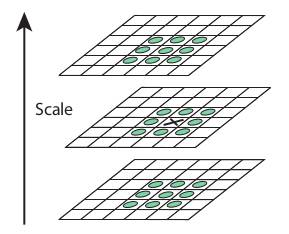
\includegraphics[width=0.4\textwidth]{img/sift_local_extrema.jpg}
        \caption{Le point d'intérêt (repéré par une croix) et son voisinage (26 voisins)}
    \end{figure}
    Si la valeur du pixel est inférieure ou supérieure à celles des 26 voisins, alors celui-ci est considéré comme un extremum local, et donc comme un point d'intérêt potentiel.
\end{frame}

\subsubsection{Chiffres clés}
\begin{frame}{Chiffres clés}
    Le papier original fournis des données empiriques permettant d'optimiser cette détection.
    \\[1cm]
    \begin{itemize}
        \item nb octaves = 4  
        \item nb flous gaussiens par octave = 5 
        \item $\sigma_{\text{init}} = 1.6$
        \item $k = \sqrt{2}$ tel que $\sigma_{\text{n+1}} = \sigma_{\text{n}}*k$ 
    \end{itemize}
\end{frame}

\subsubsection{Résultat étape 1}
\begin{frame}{Résultat étape 1}
    \begin{figure}
        \centering
        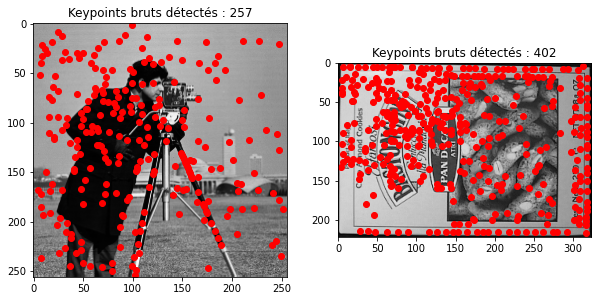
\includegraphics[width=1\textwidth]{img/etape1.png}
        \caption{Résultat de l'étape 1}
    \end{figure}
\end{frame}

\subsection{Keypoint Localization}
\begin{frame}{Keypoint Localization}
Maintenant que nous avons détecté nos Keypoints, faisont un tri pour avoir un résultat plus précis.
    \\[1cm]
    \begin{itemize}
        \item Replacer les points et éliminer le bruit  
        \item Eliminer les points sur les bords (mais pas les coins)
    \end{itemize}
\end{frame}

\subsubsection{Repositionnement et élimination du bruit}
\begin{frame}{Repositionnement et élimination du bruit}
Rappelons que le \textbf{DoG} est notée $D(x, y, \sigma)$, 
et qu'elle est obtenue par la différence de deux images floutées à des échelles proches :

\[
D(x, y, \sigma) = L(x, y, k\sigma) - L(x, y, \sigma)
\]

où $L$ est l'image convoluée avec un filtre gaussien.

\vspace{0.5cm}

On cherche les points où $D$ présente un \textbf{extremum local} (maximum ou minimum) 
dans les trois dimensions suivantes :

\begin{itemize}
    \item la position spatiale : $x, y$ ;
    \item l'échelle : $\sigma$.
\end{itemize}
\end{frame}

\begin{frame}{Repositionnement et élimination du bruit}
Pour cela, nous utilisons l'approximation de Taylor pour un candidat (développement limité):

\[
D(\mathbf{x}) \approx D + 
\frac{\partial D}{\partial \mathbf{x}}^{T} \, \hat{\mathbf{x}} +
\frac{1}{2} \, \hat{\mathbf{x}}^{T} 
\frac{\partial^{2} D}{\partial \mathbf{x}^{2}} \, \hat{\mathbf{x}}
\]

avec :

\[
\mathbf{x} = 
\begin{bmatrix}
x \\[0.2em]
y \\[0.2em]
\sigma
\end{bmatrix}
\quad \text{et} \quad
\hat{\mathbf{x}} =
\begin{bmatrix}
\Delta x \\[0.2em]
\Delta y \\[0.2em]
\Delta \sigma
\end{bmatrix}
\]

\vspace{0.4cm}

où $\hat{\mathbf{x}}$ représente le \textbf{déplacement optimal} à appliquer 
pour atteindre la position exacte de l'extrémum dans l’espace d’échelle.

\end{frame}

\begin{frame}{Repositionnement et élimination du bruit}

On cherche le point où la fonction $D(\mathbf{x})$ est \textbf{stationnaire}, c’est-à-dire :

\[
\frac{\partial D}{\partial \mathbf{x}} = 0
\]

En dérivant le développement de Taylor et en annulant la dérivée, on obtient :

\[
\frac{\partial D}{\partial \mathbf{x}} + 
\frac{\partial^{2} D}{\partial \mathbf{x}^{2}} \, \hat{\mathbf{x}} = 0
\]

d’où le \textbf{déplacement optimal} :

\[
\hat{\mathbf{x}} = 
- \left( 
\frac{\partial^{2} D}{\partial \mathbf{x}^{2}} 
\right)^{-1} 
\frac{\partial D}{\partial \mathbf{x}}
\]

\vspace{0.4cm}

Ce vecteur $\hat{\mathbf{x}}$ indique le déplacement à appliquer pour atteindre 
la position exacte de l’extrémum dans l’espace d’échelle 
(position sub-pixellaire et sub-octave).

\end{frame}

\begin{frame}{Repositionnement et élimination du bruit}
Une fois la position raffinée obtenue, on évalue la valeur de la fonction DoG 
au point ajusté $\hat{\mathbf{x}}$ à l’aide de l’approximation suivante:

\[
D(\hat{\mathbf{x}}) = D + 
\frac{1}{2} 
\frac{\partial D}{\partial \mathbf{x}}^{T} 
\hat{\mathbf{x}}
\]

\vspace{0.4cm}

Cette valeur permet de mesurer le \textbf{contraste local} du point clé.

\begin{itemize}
    \item Si $\left| D(\hat{\mathbf{x}}) \right| < 0.03$, 
    le contraste est considéré comme trop faible :
    le point est alors \textbf{rejeté} (probablement du bruit).
    \item Sinon, le point est \textbf{conservé} et servira aux étapes suivantes 
    (orientation et description).
\end{itemize}

\vspace{0.4cm}

Le seuil de $0.03$ correspond à la valeur utilisée dans le papier original.

\end{frame}


\subsubsection{Tri des coins}
\begin{frame}{Tri des coins}
SIFT utilise une approche inspirée du \textbf{détecteur de Harris}.
On analyse la \textbf{courbure locale} de l’image autour du point clé 
grâce à la \textbf{matrice Hessienne} :

\[
H = 
\begin{bmatrix}
D_{xx} & D_{xy} \\
D_{xy} & D_{yy}
\end{bmatrix}
\]

où $D_{xx}$, $D_{yy}$ et $D_{xy}$ sont les dérivées secondes 
de la fonction de différence de Gaussiennes $D(x, y)$.

\end{frame}

\begin{frame}{Tri des coins}

Les \textbf{valeurs propres} de la matrice Hessienne $H$
(désignées par $\alpha$ et $\beta$)
représentent les \textbf{courbures principales} 
dans deux directions locales :

\begin{itemize}
    \item Si $\alpha$ et $\beta$ sont \textbf{grandes et similaires} 
    $\Rightarrow$ le point se situe sur un \textbf{coin} (bon keypoint).
    \item Si une valeur est \textbf{grande} et l’autre \textbf{petite} 
    $\Rightarrow$ le point se situe sur un \textbf{bord} (mauvais keypoint).
\end{itemize}

\vspace{0.4cm}

\end{frame}

\begin{frame}{Tri des coins}

Au lieu de calculer directement les valeurs propres,
SIFT utilise un \textbf{rapport entre la trace et le déterminant} de $H$ :

\[
\frac{(\mathrm{Tr}(H))^2}{\mathrm{Det}(H)} < \frac{(r + 1)^2}{r}
\]

avec :
\[
\mathrm{Tr}(H) = D_{xx} + D_{yy}, \quad
\mathrm{Det}(H) = D_{xx}D_{yy} - D_{xy}^2
\]

\vspace{0.4cm}

Le paramètre $r$ correspond au \textbf{rapport maximal entre les courbures principales} 
($r = 10$ dans le papier).  
Si cette condition n’est pas respectée, 
le point est \textbf{rejeté} comme étant sur un bord.

\end{frame}

\subsubsection{Résultat étape 2}
\begin{frame}{Résultat étape 2}
    \begin{figure}
        \centering
        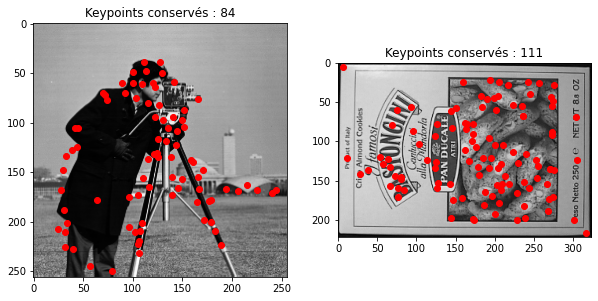
\includegraphics[width=1\textwidth]{img/etape2.png}
        \caption{Résultat de l'étape 2}
    \end{figure}
\end{frame}

\subsection{Orientation Assignment}
\begin{frame}{Orientation Assignment}  
Maintenant que les \textit{keypoints} ont été détectés et raffinés, 
il faut leur attribuer une \textbf{orientation} afin de rendre la description 
\textbf{invariante à la rotation} de l’image.

\vspace{0.4cm}

Pour pouvoir comparer (ou \textit{matcher}) deux points clés provenant 
d’images différentes, il faut que leur description soit indépendante :
\\
\begin{itemize}
    \item de la rotation,
    \item de l’échelle,
    \item et partiellement des changements d’éclairage.
\end{itemize}

\vspace{0.4cm}

Cette étape vise donc à définir une \textbf{direction dominante}
pour chaque point clé, qui servira de repère 
pour la création du descripteur.

\end{frame}

\begin{frame}{Attribution de l'orientation dominante}

Pour chaque point clé détecté :

\begin{itemize}
    \item On extrait une \textbf{voisinage local} autour du point, 
    dont la taille dépend de son \textbf{échelle}.

    \item On calcule le \textbf{gradient d’intensité} des points de cette région. 
\end{itemize}

\end{frame}

\begin{frame}{Attribution de l'orientation dominante}
\begin{itemize}
    
    
    \item Les orientations des gradients sont ajoutées dans un 
    \textbf{histogramme de 36 bins} couvrant $360^\circ$, 
    pondéré par :
    \begin{itemize}
        \item la \textbf{magnitude du gradient}
        \item une \textbf{fenêtre gaussienne} centrée sur le point clé pour favoriser les points les plus proches 
        (écart-type $1.5 \times$ l’échelle du keypoint).
        \begin{figure}
            \centering
            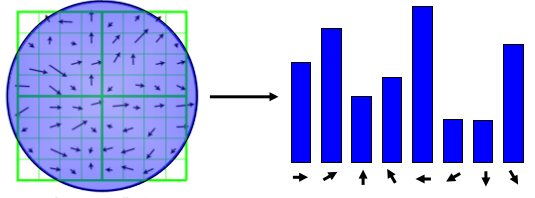
\includegraphics[width=0.58\textwidth]{img/orientation.png}
        \caption{Histogramme des orientation du voisinage}
    \end{figure}
    \end{itemize}

    \item Le \textbf{pic de l'histogramme} indique l’orientation principale.  
    Toute autre orientation ayant une amplitude supérieure à $80\%$ du pic 
    est aussi conservée pour créer des keypoints supplémentaires.
\end{itemize}
    
\end{frame}

\subsubsection{Résultat étape 3}
\begin{frame}{Résultat étape 3}
    \begin{figure}
        \centering
        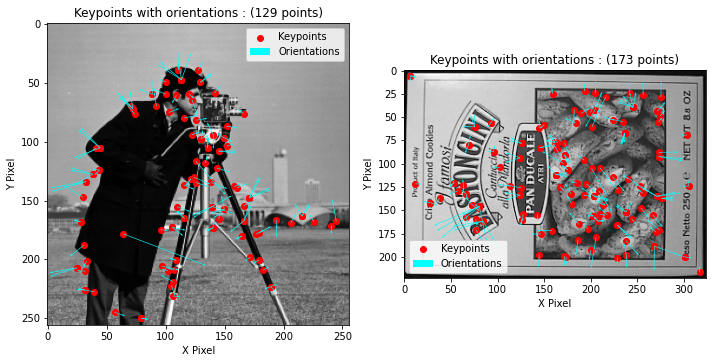
\includegraphics[width=1\textwidth]{img/etape3.png}
        \caption{Résultat de l'étape 3}
    \end{figure}
\end{frame}


\subsection{Keypoints descriptor}
\begin{frame}{Keypoints descriptor}
    Enfin, nous allons créer les \textbf{descripteurs des points d'intérêt}
selon la méthode SIFT.

\vspace{0.4cm}

Pour cela, on considère une \textbf{fenêtre carrée} de taille 
$12\sigma \times 12\sigma$ pixels, centrée autour d'un point d'intérêt
et proportionnelle à son niveau de flou de détection $\sigma$.

\vspace{0.3cm}

Cette grande fenêtre est ensuite \textbf{découpée en 16 petites fenêtres carrées},
chacune de taille $3\sigma \times 3\sigma$ pixels.

\end{frame}

\begin{frame}{Construction des histogrammes locaux}

Pour chacune des 16 sous-fenêtres :

\begin{itemize}
    \item Un \textbf{histogramme des orientations du gradient} est construit 
    de la même manière que dans l’étape précédente.

    \item Cette fois, les orientations sont exprimées \textbf{relativement à l’orientation du point d’intérêt} :  
    chaque orientation locale est soustraite de l’orientation dominante du keypoint.

    \item Chaque histogramme contient \textbf{8 classes}, 
    soit des intervalles de $45^\circ$.
\end{itemize}

\end{frame}

\begin{frame}{Formation du vecteur descripteur}

Chaque sous-fenêtre produit un histogramme comportant \textbf{8 valeurs}.

\vspace{0.3cm}

Ainsi, les 16 sous-fenêtres fournissent au total :
\[
16 \text{ sous-fenêtres} \times 8 \text{ valeurs} = 128 \text{ composantes.}
\]

\vspace{0.3cm}

Ces 128 valeurs sont concaténées pour former un \textbf{vecteur de dimension 128}.

    \begin{figure}
        \centering
        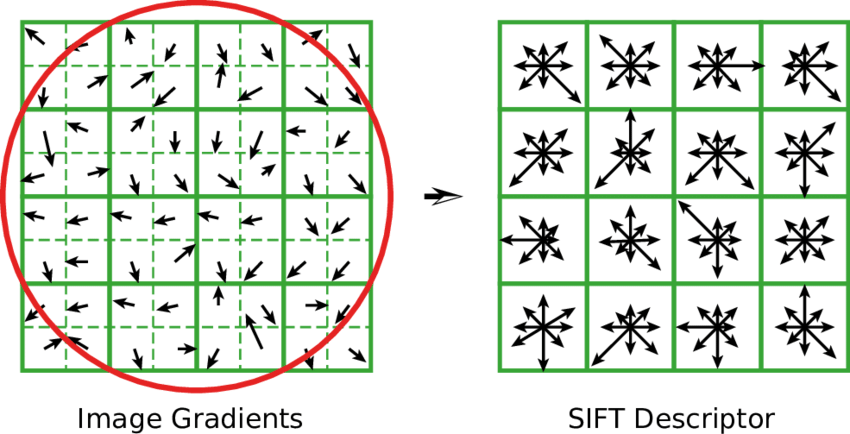
\includegraphics[width=0.5\textwidth]{img/SIFT-descriptor-The-well-known-SIFT-descriptor-consists-of-3D-histograms-of-image.png}
        \caption{Histogramme d'une sous fenetre}
    \end{figure}

\end{frame}

\section{Les limites de SIFT}
\begin{frame}{Limites et inconvénients de l'algorithme}

    \begin{itemize}
        \item \textbf{1. Coût de calcul élevé (Temps réel difficile)}
		\\        
        Il est souvent trop lent pour des applications temps réel embarquées comparé à des alternatives comme \textit{ORB} ou \textit{SURF}.
        
        \vspace{0.3cm} % Petit espace pour aérer
        
        \item \textbf{2. Descripteurs volumineux (128 dimensions)}
		\\        
        Cela ralentit considérablement l'étape de matching sur de grandes bases de données.
        
        \vspace{0.3cm}
        
        \item \textbf{3. Limite de description}
		\\        
        Dans des images trop peu détaillées (comme des codes ARUCO ou des QR codes), la description des images n'est pas assez complexe pour faire un matching efficace.

    \end{itemize}
\end{frame}

\section{Exemples d'applications}
\subsection{Multiples applications}
\begin{frame}{Liste non exaustive d'exemples}
    \begin{itemize}
        \item Parttern matching  
        \item Mosaïquage / Panoramique (Image Stitching)
        \item Reconnaissance d’objets
        \item Réalité augmentée
        \item Classification d'image
        \item etc ...
    \end{itemize}
\end{frame}

\subsection{Pattern matching}
\begin{frame}{Pattern matching}
    Identifier un objet spécifique au sein d'une image ou d'une base de données d'images.
    \begin{figure}
        \centering
        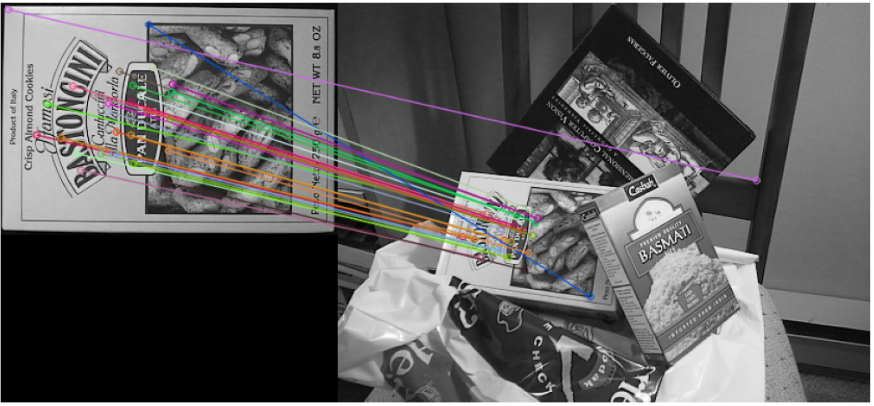
\includegraphics[width=0.8\textwidth]{img/application_pattern_matching.png}
        \caption{Exemple de pattern matching}
    \end{figure}
    Application : 
    \begin{itemize}
        \item Systèmes de reconnaissance d'objets
        \item Vérification d'images
    \end{itemize}
\end{frame}

\subsection{Correspondance et Assemblage d'Images}
\begin{frame}{Correspondance et Assemblage d'Images}
    Trouver des points communs entre des images qui se chevauchent.
    \begin{figure}[h!]
    \centering
    \begin{minipage}{0.48\textwidth}
        \centering
        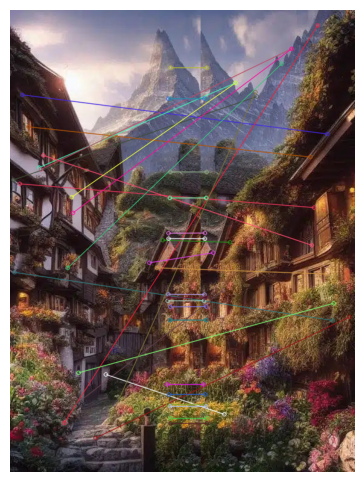
\includegraphics[width=0.6\linewidth]{img/application_stitching_1.png}
        \caption{Identification des points communs entre deux images}
    \end{minipage}
    \hfill
    \begin{minipage}{0.48\textwidth}
        \centering
        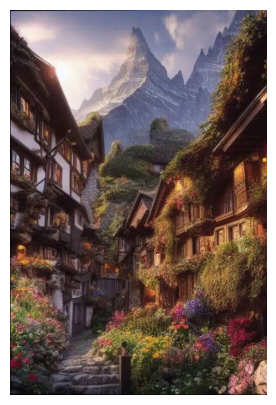
\includegraphics[width=0.55\linewidth]{img/application_stitching_2.png}
        \caption{Image reconstituée après stitching}
    \end{minipage}
\end{figure}
Application : 
    \begin{itemize}
        \item Assemblage de panoramas
        \item Appariement stéréoscopique
    \end{itemize}
\end{frame}

\subsection{Reconstruction et Modélisation 3D}
\begin{frame}{Reconstruction et Modélisation 3D}
    Obtenir des informations géométriques d'une scène ou d'un objet à partir de plusieurs images 2D.
    \begin{figure}
        \centering
        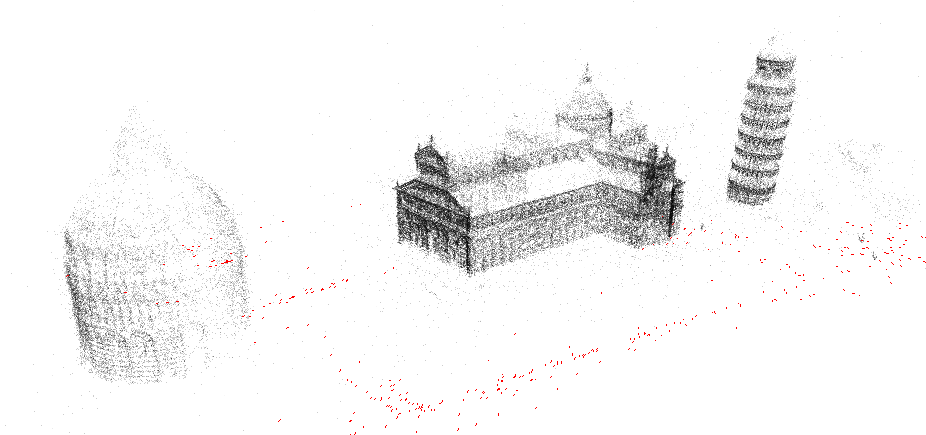
\includegraphics[width=0.8\textwidth]{img/application_sfm.png}
        \caption{Reconstruction 3D de la tour de Pise à partir de multiples images 2D}
    \end{figure}
    Application : 
    \begin{itemize}
        \item Reconstruction 3D
        \item Réalité Augmentée
    \end{itemize}
\end{frame}

\subsection{Robotique et Navigation}
\begin{frame}{Robotique et Navigation}
    Permettre à un robot de comprendre son environnement et sa propre position.
    \begin{figure}
        \centering
        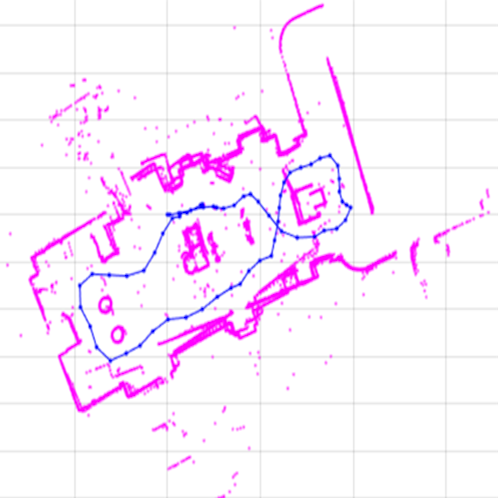
\includegraphics[width=0.35\textwidth]{img/application_slam.png}
        \caption{Map de l'environnement créée par un robot}
    \end{figure}
    Application : 
    \begin{itemize}
        \item Localisation et Cartographie Simultanées (SLAM)
        \item Suivi d'objets
    \end{itemize}
\end{frame}

\end{document}

